% SolarMax wiring diagrams
% Compile:  pdflatex wiring_diagram.tex   (run from docs/)
% Produces: page 1 = legend + power wiring, page 2 = signal/sensor wiring.

\documentclass[landscape,a4paper]{article}
\usepackage[margin=1cm,landscape]{geometry}
\usepackage{tikz}
\usepackage{xcolor}
\usepackage{adjustbox}
\usetikzlibrary{matrix,positioning,calc}
\pagestyle{empty}

% ---- Wire net colors (one color per electrical net type) --------------------
\definecolor{net12v}{HTML}{D32F2F}   % 12 V +      red
\definecolor{netgnd}{HTML}{212121}   % GND         near-black
\definecolor{net5v}{HTML}{F57C00}    % 5 V         orange
\definecolor{net3v3}{HTML}{FBC02D}   % 3.3 V       yellow
\definecolor{netmot}{HTML}{6A1B9A}   % motor out   purple
\definecolor{netpwm}{HTML}{1565C0}   % PWM/EN      blue
\definecolor{neti2c}{HTML}{2E7D32}   % I2C         green
\definecolor{netlim}{HTML}{C2185B}   % limits      magenta
\definecolor{netanem}{HTML}{00838F}  % anemometer  cyan
\definecolor{netana}{HTML}{5D4037}   % analog      brown

% ---- Styles -----------------------------------------------------------------
\tikzset{
  modlabel/.style={font=\bfseries\small},
  mod/.style={matrix of nodes, draw, rounded corners, inner sep=3pt,
    nodes={draw, anchor=center, minimum width=#1, minimum height=0.62cm,
           font=\footnotesize, fill=white},
    row sep=-\pgflinewidth, column sep=-\pgflinewidth},
  mod/.default=2.6cm,
  wire/.style={line width=1.1pt},
  pwr/.style={line width=2pt},
}

\newcommand{\legendbox}[2]{\tikz\draw[line width=2.4pt,#1](0,0)--(0.7,0);\,#2}

\begin{document}

\begin{center}{\Large\bfseries SolarMax — Wiring Diagrams}\\[2pt]
\small Colored wires by net. All grounds are common. Pin names match \texttt{include/config.h}.\end{center}

\noindent\fbox{\parbox{\dimexpr\textwidth-2\fboxsep-2\fboxrule\relax}{%
\textbf{Wire color legend:}\quad
\legendbox{net12v}{+12\,V}\quad
\legendbox{netgnd}{GND}\quad
\legendbox{net5v}{+5\,V}\quad
\legendbox{net3v3}{+3.3\,V}\quad
\legendbox{netmot}{Motor out}\quad
\legendbox{netpwm}{Motor PWM/EN}\quad
\legendbox{neti2c}{I\textsuperscript{2}C}\quad
\legendbox{netlim}{Limit switch}\quad
\legendbox{netanem}{Anemometer sig}\quad
\legendbox{netana}{Analog (pot/LDR)}%
}}

\vspace{6pt}
\begin{center}{\large\bfseries 1. Power Distribution}\end{center}

\begin{adjustbox}{max width=\textwidth, max totalheight=0.78\textheight, center}
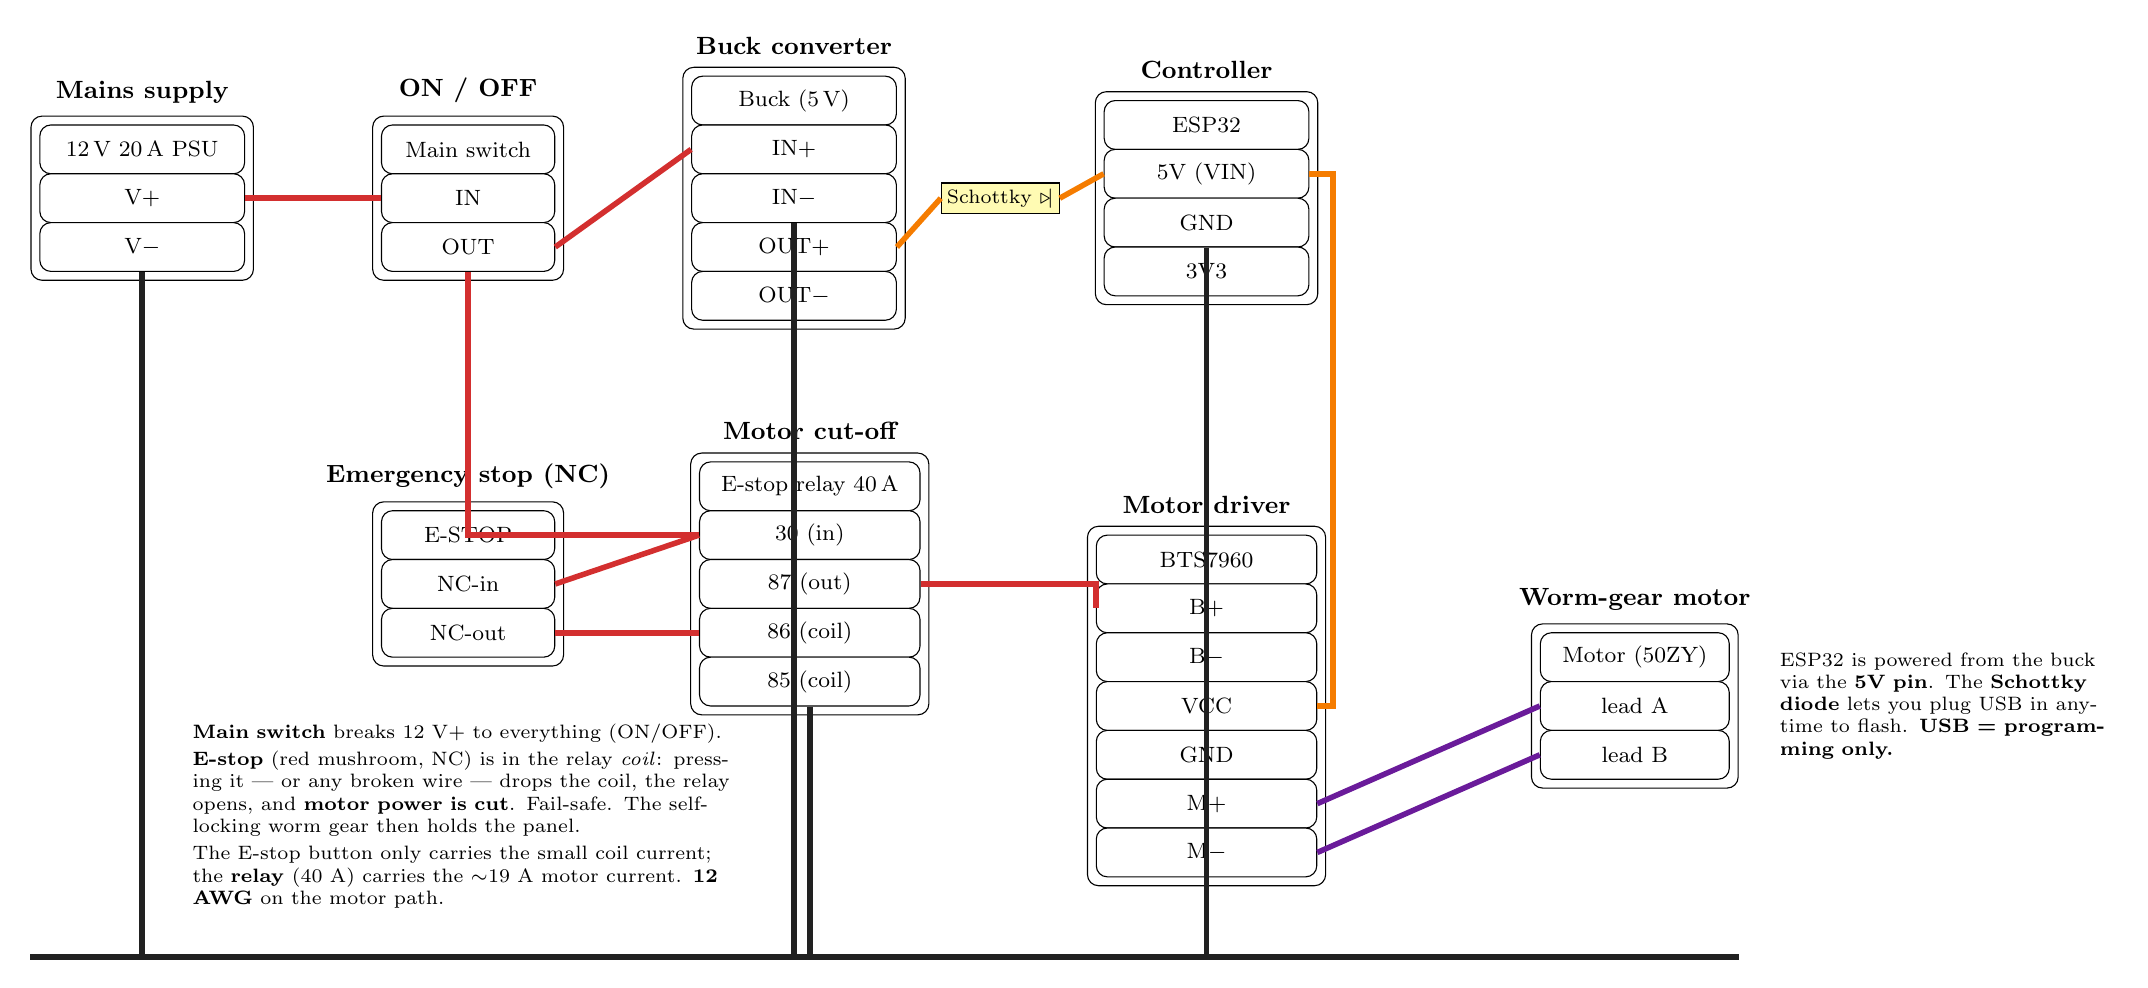
\begin{tikzpicture}

\matrix[mod=2.6cm] (psu) { 12\,V 20\,A PSU \\ V+ \\ V$-$ \\ };
\node[modlabel, above=1pt of psu] {Mains supply};

\matrix[mod=2.2cm, right=1.5cm of psu] (msw) { Main switch \\ IN \\ OUT \\ };
\node[modlabel, above=1pt of msw] {ON / OFF};

\matrix[mod=2.6cm, right=1.5cm of msw] (buck)
  { Buck (5\,V) \\ IN+ \\ IN$-$ \\ OUT+ \\ OUT$-$ \\ };
\node[modlabel, above=1pt of buck] {Buck converter};

\matrix[mod=2.6cm, right=2.4cm of buck] (esp)
  { ESP32 \\ 5V (VIN) \\ GND \\ 3V3 \\ };
\node[modlabel, above=1pt of esp] {Controller};

\matrix[mod=2.2cm, below=2.8cm of msw] (estop) { E-STOP \\ NC-in \\ NC-out \\ };
\node[modlabel, above=1pt of estop] {Emergency stop (NC)};

\matrix[mod=2.8cm, right=1.6cm of estop] (rly)
  { E-stop relay 40\,A \\ 30 (in) \\ 87 (out) \\ 86 (coil) \\ 85 (coil) \\ };
\node[modlabel, above=1pt of rly] {Motor cut-off};

\matrix[mod=2.8cm, below=2.8cm of esp] (bts)
  { BTS7960 \\ B+ \\ B$-$ \\ VCC \\ GND \\ M+ \\ M$-$ \\ };
\node[modlabel, above=1pt of bts] {Motor driver};

\matrix[mod=2.4cm, right=2.6cm of bts] (mot)
  { Motor (50ZY) \\ lead A \\ lead B \\ };
\node[modlabel, above=1pt of mot] {Worm-gear motor};

% ===== 12 V + (red) =====
\draw[pwr,net12v] (psu-2-1.east) -- (msw-2-1.west);                 % PSU V+ -> MAIN IN
\draw[pwr,net12v] (msw-3-1.east) -- (buck-2-1.west);               % MAIN OUT -> buck IN+
\draw[pwr,net12v] (msw-3-1.south) |- (rly-2-1.west);              % MAIN OUT -> relay 30
\draw[pwr,net12v] (rly-2-1.west) -- (estop-2-1.east);            % relay 30 (switched V+) -> E-stop NC-in
\draw[pwr,net12v] (estop-3-1.east) |- (rly-4-1.west);            % E-stop NC-out -> relay 86 (coil)
\draw[pwr,net12v] (rly-3-1.east) -| (bts-2-1.west);              % relay 87 -> BTS B+

% ===== GND bus (black) — common ground =====
\coordinate (gy) at ([yshift=-0.9cm]bts.south);
\draw[pwr,netgnd] (psu.west |- gy) -- (mot.east |- gy);
\foreach \p in {psu-3-1, buck-3-1, buck-5-1, esp-3-1, bts-3-1, bts-5-1, rly-5-1}
  { \draw[pwr,netgnd] (\p.south) -- (\p.south |- gy); }

% ===== 5 V (orange) — buck -> Schottky diode -> ESP 5V pin =====
\node[draw,fill=yellow!30,font=\scriptsize,inner sep=2pt] (d5) at ($(buck.east)!0.5!(esp.west)$) {Schottky $\triangleright\!|$};
\draw[pwr,net5v] (buck-4-1.east) -- (d5.west);
\draw[pwr,net5v] (d5.east) -- (esp-2-1.west);
\draw[pwr,net5v] (esp-2-1.east) -- ++(0.3,0) |- (bts-4-1.east);   % ESP 5V -> BTS VCC

% ===== Motor (purple) =====
\draw[pwr,netmot] (bts-6-1.east) -- (mot-2-1.west);
\draw[pwr,netmot] (bts-7-1.east) -- (mot-3-1.west);

\node[align=left, font=\scriptsize, below=0.6cm of estop, text width=7cm]
  {\textbf{Main switch} breaks 12 V+ to everything (ON/OFF).\\[2pt]
   \textbf{E-stop} (red mushroom, NC) is in the relay \emph{coil}: pressing it — or any broken
   wire — drops the coil, the relay opens, and \textbf{motor power is cut}. Fail-safe. The
   self-locking worm gear then holds the panel.\\[2pt]
   The E-stop button only carries the small coil current; the \textbf{relay} (40 A) carries the
   $\sim$19 A motor current. \textbf{12 AWG} on the motor path.};

\node[align=left, font=\scriptsize, right=0.4cm of mot, text width=4.2cm]
  {ESP32 is powered from the buck via the \textbf{5V pin}. The \textbf{Schottky diode} lets you
   plug USB in anytime to flash. \textbf{USB = programming only.}};

\end{tikzpicture}
\end{adjustbox}

% =============================================================================
\newpage
\begin{center}{\large\bfseries 2. Control, Sensor \& Power/Ground Wiring}\\[1pt]
\small Signal wires go left to the ESP32. Every power and ground pin is shown on the right
with a colored tag. \textbf{All GND tags are the same common ground.}\end{center}

\begin{adjustbox}{max width=\textwidth, max totalheight=0.86\textheight, center}
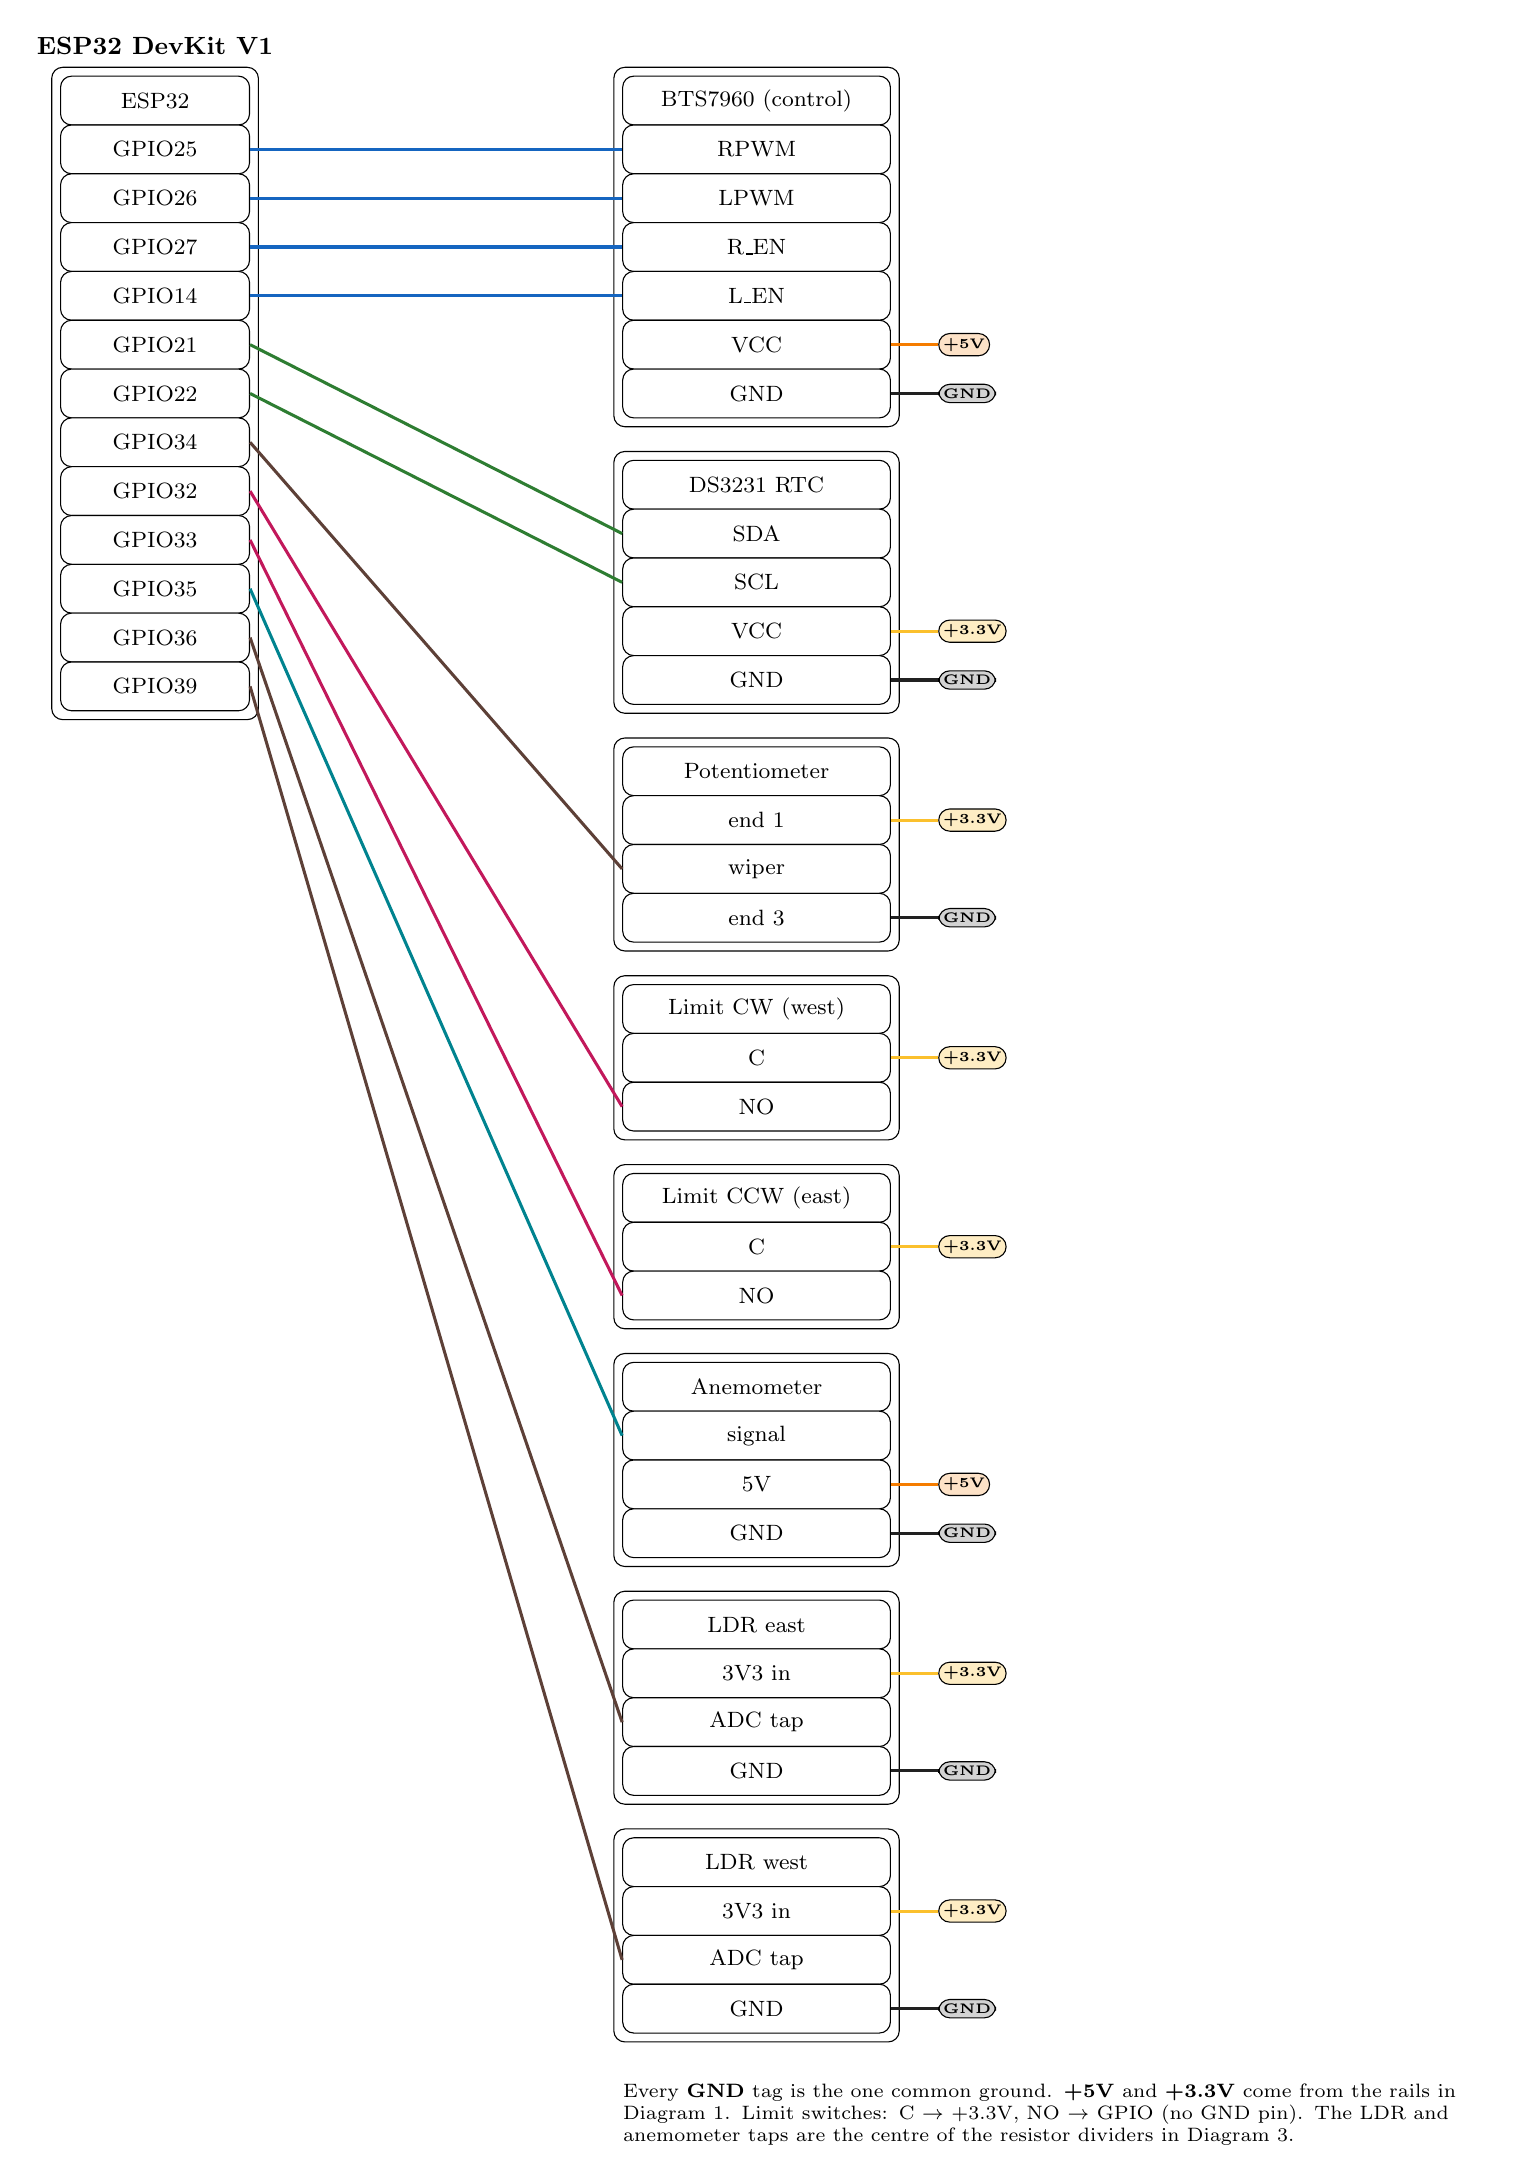
\begin{tikzpicture}[
  tagG/.style={draw,rounded corners,font=\tiny\bfseries,inner sep=1.6pt,fill=netgnd!20},
  tag3/.style={draw,rounded corners,font=\tiny\bfseries,inner sep=1.6pt,fill=net3v3!28},
  tag5/.style={draw,rounded corners,font=\tiny\bfseries,inner sep=1.6pt,fill=net5v!22}]

\matrix[mod=2.4cm] (e)
  { ESP32 \\ GPIO25 \\ GPIO26 \\ GPIO27 \\ GPIO14 \\ GPIO21 \\ GPIO22 \\
    GPIO34 \\ GPIO32 \\ GPIO33 \\ GPIO35 \\ GPIO36 \\ GPIO39 \\ };
\node[modlabel, above=1pt of e] {ESP32 DevKit V1};

\matrix[mod=3.4cm, right=4.5cm of e.north east, anchor=north west] (drv)
  { BTS7960 (control) \\ RPWM \\ LPWM \\ R\_EN \\ L\_EN \\ VCC \\ GND \\ };
\matrix[mod=3.4cm, below=3mm of drv] (rtc) { DS3231 RTC \\ SDA \\ SCL \\ VCC \\ GND \\ };
\matrix[mod=3.4cm, below=3mm of rtc] (pot) { Potentiometer \\ end 1 \\ wiper \\ end 3 \\ };
\matrix[mod=3.4cm, below=3mm of pot] (lcw) { Limit CW (west) \\ C \\ NO \\ };
\matrix[mod=3.4cm, below=3mm of lcw] (lccw){ Limit CCW (east) \\ C \\ NO \\ };
\matrix[mod=3.4cm, below=3mm of lccw](anem){ Anemometer \\ signal \\ 5V \\ GND \\ };
\matrix[mod=3.4cm, below=3mm of anem](ldre){ LDR east \\ 3V3 in \\ ADC tap \\ GND \\ };
\matrix[mod=3.4cm, below=3mm of ldre](ldrw){ LDR west \\ 3V3 in \\ ADC tap \\ GND \\ };

% ---- signal wires (ESP -> peripheral, left side) ----
\draw[wire,netpwm] (e-2-1.east) -- (drv-2-1.west);
\draw[wire,netpwm] (e-3-1.east) -- (drv-3-1.west);
\draw[wire,netpwm] (e-4-1.east) -- (drv-4-1.west);
\draw[wire,netpwm] (e-5-1.east) -- (drv-5-1.west);
\draw[wire,neti2c] (e-6-1.east) -- (rtc-2-1.west);
\draw[wire,neti2c] (e-7-1.east) -- (rtc-3-1.west);
\draw[wire,netana] (e-8-1.east) -- (pot-3-1.west);
\draw[wire,netlim] (e-9-1.east)  -- (lcw-3-1.west);
\draw[wire,netlim] (e-10-1.east) -- (lccw-3-1.west);
\draw[wire,netanem] (e-11-1.east) -- (anem-2-1.west);
\draw[wire,netana] (e-12-1.east) -- (ldre-3-1.west);
\draw[wire,netana] (e-13-1.east) -- (ldrw-3-1.west);

% ---- power / ground tags (peripheral -> tag, right side) ----
% +5V
\node[tag5,right=6mm of drv-6-1](t1){+5V};  \draw[wire,net5v](drv-6-1.east)--(t1.west);
\node[tag5,right=6mm of anem-3-1](t2){+5V}; \draw[wire,net5v](anem-3-1.east)--(t2.west);
% +3.3V
\node[tag3,right=6mm of rtc-4-1](t3){+3.3V};  \draw[wire,net3v3](rtc-4-1.east)--(t3.west);
\node[tag3,right=6mm of pot-2-1](t4){+3.3V};  \draw[wire,net3v3](pot-2-1.east)--(t4.west);
\node[tag3,right=6mm of lcw-2-1](t5){+3.3V};  \draw[wire,net3v3](lcw-2-1.east)--(t5.west);
\node[tag3,right=6mm of lccw-2-1](t6){+3.3V}; \draw[wire,net3v3](lccw-2-1.east)--(t6.west);
\node[tag3,right=6mm of ldre-2-1](t7){+3.3V}; \draw[wire,net3v3](ldre-2-1.east)--(t7.west);
\node[tag3,right=6mm of ldrw-2-1](t8){+3.3V}; \draw[wire,net3v3](ldrw-2-1.east)--(t8.west);
% GND  (all the same common ground)
\node[tagG,right=6mm of drv-7-1](g1){GND};  \draw[wire,netgnd](drv-7-1.east)--(g1.west);
\node[tagG,right=6mm of rtc-5-1](g2){GND};  \draw[wire,netgnd](rtc-5-1.east)--(g2.west);
\node[tagG,right=6mm of pot-4-1](g3){GND};  \draw[wire,netgnd](pot-4-1.east)--(g3.west);
\node[tagG,right=6mm of anem-4-1](g4){GND}; \draw[wire,netgnd](anem-4-1.east)--(g4.west);
\node[tagG,right=6mm of ldre-4-1](g5){GND}; \draw[wire,netgnd](ldre-4-1.east)--(g5.west);
\node[tagG,right=6mm of ldrw-4-1](g6){GND}; \draw[wire,netgnd](ldrw-4-1.east)--(g6.west);

\node[font=\scriptsize,align=left,below=4mm of ldrw.south west,anchor=north west,text width=11cm]
 {Every \textbf{GND} tag is the one common ground. \textbf{+5V} and \textbf{+3.3V} come from the
  rails in Diagram 1. Limit switches: C $\to$ +3.3V, NO $\to$ GPIO (no GND pin). The LDR and
  anemometer taps are the centre of the resistor dividers in Diagram 3.};

\end{tikzpicture}
\end{adjustbox}

% =============================================================================
\newpage
\begin{center}{\large\bfseries 3. Voltage Divider Details}\\[1pt]
\small Two sensors need a resistor divider. Build these exactly — they protect the
ESP32 and set the correct readings.\end{center}

\vspace{1cm}
\begin{adjustbox}{max width=\textwidth, center}
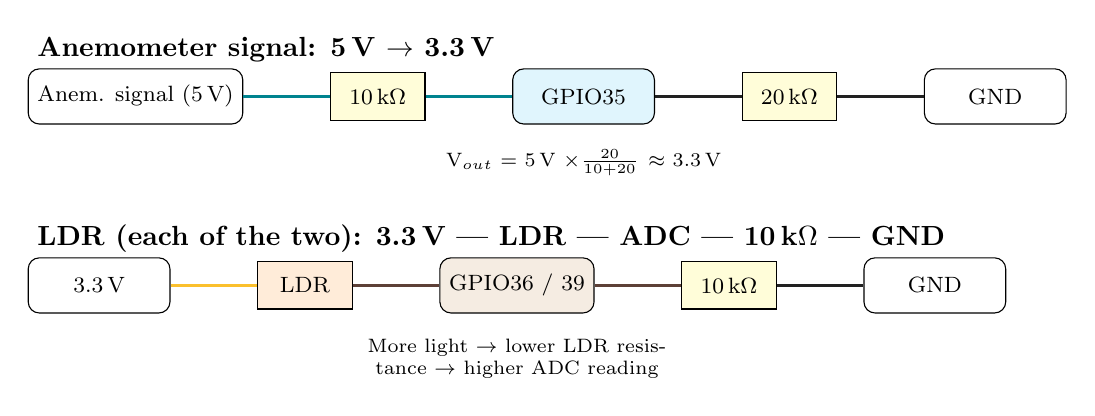
\begin{tikzpicture}[
  pinnode/.style={draw, rounded corners, minimum height=0.7cm, minimum width=1.8cm,
                  font=\footnotesize, fill=white},
  res/.style={draw, fill=yellow!15, minimum height=0.6cm, minimum width=1.2cm, font=\footnotesize},
  node distance=1.1cm]

% ---- Anemometer divider ----
\node[font=\bfseries] (atitle) {Anemometer signal: 5\,V $\rightarrow$ 3.3\,V};
\node[pinnode, below=0.6cm of atitle.west, anchor=west] (asig) {Anem. signal (5\,V)};
\node[res, right=of asig] (ar1) {10\,k$\Omega$};
\node[pinnode, right=of ar1, fill=cyan!12] (agpio) {GPIO35};
\node[res, right=of agpio] (ar2) {20\,k$\Omega$};
\node[pinnode, right=of ar2] (agnd) {GND};
\draw[wire,netanem] (asig.east) -- (ar1.west);
\draw[wire,netanem] (ar1.east) -- (agpio.west);
\draw[wire,netgnd]  (agpio.east) -- (ar2.west);
\draw[wire,netgnd]  (ar2.east) -- (agnd.west);
\node[font=\scriptsize, below=0.2cm of agpio, text width=4cm, align=center]
  {V$_{out}$ = 5\,V $\times\frac{20}{10+20}\approx$ 3.3\,V};

% ---- LDR divider ----
\node[font=\bfseries, below=2.4cm of atitle.west, anchor=west] (ltitle) {LDR (each of the two): 3.3\,V — LDR — ADC — 10\,k$\Omega$ — GND};
\node[pinnode, below=0.6cm of ltitle.west, anchor=west] (l3v3) {3.3\,V};
\node[res, right=of l3v3, fill=orange!15] (lldr) {LDR};
\node[pinnode, right=of lldr, fill=brown!15] (ladc) {GPIO36 / 39};
\node[res, right=of ladc] (lr) {10\,k$\Omega$};
\node[pinnode, right=of lr] (lgnd) {GND};
\draw[wire,net3v3] (l3v3.east) -- (lldr.west);
\draw[wire,netana] (lldr.east) -- (ladc.west);
\draw[wire,netana] (ladc.east) -- (lr.west);
\draw[wire,netgnd] (lr.east) -- (lgnd.west);
\node[font=\scriptsize, below=0.2cm of ladc, text width=5cm, align=center]
  {More light $\rightarrow$ lower LDR resistance $\rightarrow$ higher ADC reading};

\end{tikzpicture}
\end{adjustbox}

\end{document}
